\begin{figure}[p]
  \centering
  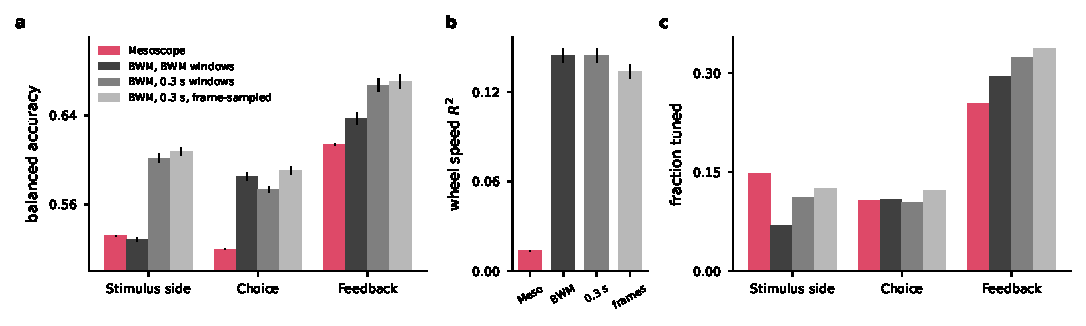
\includegraphics[width=7.00in,height=0.78\textheight,keepaspectratio]{si/si_windows_panels.pdf}
  \caption{Do the analysis windows or the mesoscope's slow sampling explain the BWM vs mesoscope differences? The same BWM units are re-analysed (i) with the mesoscope windows ($[0, 0.3]$\,s after stimulus onset, $[-0.3, 0]$\,s before movement onset, $[0, 0.3]$\,s after feedback) and (ii) additionally frame-sampled: spikes are binned into 0.205\,s frames (the mesoscope frame period) and the resulting rate trace is read out exactly like a mesoscope trace (linear interpolation between frame centres, mean over the window). \textbf{a} Decoding from 10 neurons per session and 0.4\,mm bin (mean $\pm$ s.e.m. over session $\times$ bin pairs), binary variables. \textbf{b} Same for wheel speed ($R^2$). The wheel bins are 0.2\,s in all versions; the frame-sampled version reads them from the frame-resolution trace. \textbf{c} Fraction of neurons significantly tuned ($p<0.05$), same test as in the main figure.}
  \label{fig:si_windows}
\end{figure}
